%Template_made_by_SGjTeX

\documentclass[a4paper,13pt]{book}
\usepackage[utf8]{inputenc}     
\usepackage[T1]{fontenc}
\usepackage{amsmath,amsthm, amssymb,xcolor,amsfonts,mathrsfs} 
\usepackage[left=2.5cm,right=2.5cm,top=2.5cm,bottom=2.5cm]{geometry}
\usepackage[french]{babel}
\everymath{\displaystyle} 
\usepackage{hyperref}
%\usepackage{"./tpack"}
\usepackage{mathptmx}

\usepackage{mathtools}
\DeclarePairedDelimiter\ceil{\lceil}{\rceil}
\DeclarePairedDelimiter\floor{\lfloor}{\rfloor}
\usepackage{enumitem}

\usepackage{pgfplots} % Package pour tracer les courbes
\usepackage{filecontents} % Permet d'intégrer les données dans le fichier source
\usepackage[explicit]{ titlesec}
\usepackage{fancybox}
%\usepackage{thmbox}   
%================================ 
\usepackage{fancyhdr}
\usepackage{fancybox}

\usepackage{xcolor}
\pagestyle{fancy}
\fancyhf{} 

%\fancyfoot[RO,LE]{\rightmark} 

\cfoot{\thepage}
\lfoot{}
\renewcommand{\chaptermark}[1]{\markboth{#1}{}}
%===============================
\newtheorem{definition}{Définition}[section]
\newtheorem{theo}{Théorème}[section]
\newtheorem{pro}{Proposition}[section] 
\newtheorem{cor}{Corollaire}[section]
\newtheorem{lem}{Lemme}[section]
\newtheorem{rem}{Remarque}[section]

\definecolor{gris}{gray}{0.9}
\definecolor{perfectorange}{RGB}{255,165,20}
\definecolor{darkblue}{RGB}{25,25,100}
\definecolor{darkkblue}{RGB}{0,0,50}
\definecolor{darkred}{RGB}{180,0,0}
\definecolor{green_identifiers}{RGB}{00,80,00}
\definecolor{blue_know}{RGB}{00,20,20}
\definecolor{orange_comments}{RGB}{214, 161, 126}
\definecolor{red_keywords}{RGB}{215, 103, 129}
\definecolor{black_strings}{RGB}{50, 50, 50}
%utilis� dans la partie analyse
\definecolor{fond}{rgb}{.55,.55,.92}
%fin creation couleurs
% Définir le théorème avec couleur rouge
\newtheorem{danger1}{Attention}[section]
\newenvironment{danger}{\begin{danger1}\color{darkred}}{\end{danger1}}

% Définir le théorème avec couleur verte
\newtheorem{know1}{A Savoir}[section]
\newenvironment{know}{\begin{know1}\color{blue_know}}{\end{know1}}

\renewcommand{\footrulewidth}{1pt} 
\renewcommand{\thesection}{\arabic{section}}
\renewcommand{\thesubsection}{\thesection.\arabic{subsection}}
\renewcommand{\thesubsubsection}{\thesubsection.\arabic{subsubsection}}

\newcommand{\Hrule}{
	\rule{\linewidth}{0.5mm}
}
\newcommand\justify{%
  \let\\\@centercr
  \rightskip\z@skip
  \leftskip\z@skip}
%%===exercices 
%\newcounter{ex}
\newenvironment{exe}% exple \begin{exe}...\end{exe}
{\refstepcounter{ex}%
	\par\noindent
	{\underline{\bfseries{Exercice \theex \hspace*{0.009 cm} :}} }
	\mdseries
	\slshape}
{\par
	\medskip}
%====exemples
\newcounter{exple}
\newenvironment{exple}
{\refstepcounter{exple}%
	\par\noindent
	{\underline{\bfseries{Exemple  :}} }
	\mdseries
	\slshape}
{\par
	\medskip}
%====preuve
%\newenvironment{proof}
%{\rmfamily\mdseries{\bfseries Preuve : }}
%{\hfill$\blacksquare$}
%======
\renewcommand{\baselinestretch}{1.3}  

%%%%%%%%%%%%%%%%%%%%%%%%%%%%%%%%%

\newcommand{\ps}[2]{\left\langle #1 ,#2 \right\rangle  }
%%%%%%%%%%%%%%%%%%%%%% 
\let\cleardoublepage\clearpage 

\usepackage[explicit]{titlesec}
\usepackage{minitoc}
\renewcommand{\mtctitle}{Plan}
\usepackage[most]{tcolorbox}
\newcommand\mychapter{\titleformat{\chapter}[block]{}{}{0pt}{\centering\hrule height 5pt
		\vglue-1.1 \baselineskip
		\tcbox[enhanced,colback=white,frame code={}]{\bfseries\chaptername\hskip2mm \thechapter}
		\bigskip
		\vglue-3mm\hrule \vglue3mm
		{\huge \bfseries ##1}\vglue3mm\hrule
	}[]\chapter}
\dominitoc
\usepackage{caption}
\usepackage{listings}

%%configuration de listings
\definecolor{codegreen}{rgb}{0,0.6,0}
\definecolor{codegray}{rgb}{0.5,0.5,0.5}
\definecolor{codepurple}{rgb}{0.58,0,0.82}
\definecolor{backcolour}{rgb}{0.97,0.99,0.99}

\lstdefinestyle{mystyle}{
    backgroundcolor=\color{backcolour},
    commentstyle=\color{codegreen},
    keywordstyle=\color{magenta},
    numberstyle=\tiny\color{codegray},
    stringstyle=\color{codepurple},
    basicstyle=\ttfamily\footnotesize,
    breakatwhitespace=false,
    breaklines=true,
    captionpos=b,
    keepspaces=true,
    numbers=left,
    numbersep=5pt,
    showspaces=false,
    showstringspaces=false,
    showtabs=false,
    tabsize=4
}

\lstset{style=mystyle}

\definecolor{Zgris}{rgb}{238, 238, 238}

\newsavebox{\BBbox}
\newenvironment{DDbox}[1]{
\begin{lrbox}{\BBbox}\begin{minipage}{\linewidth}}
{\end{minipage}\end{lrbox}\noindent\colorbox{Zgris}{\usebox{\BBbox}} \\
[.5cm]}
\author{\bsc{DADA SIMEU Cédric Darel}}


\begin{document}
	\graphicspath{ {../template_page_garde} }

\begin{center}
  
\includegraphics[scale=0.15]{logo.jpg}
\end{center}

{\vspace{7em}}

\begin{center}
  \begin{tabular}{|lp{5.0cm}lll|}
    \hline
    &  &  &  & {\small{2024/25}}\\
    &  &  &  & \\
    &  &  &  & \\
    \textbf{Nom:} & \bsc{DADA SIMEU Cédric Darel}
    
    \  &  &  & \\
    \textbf{Email:} & cedric-darel.dada@ensta-paris.fr
    
    \  &  &  & \\
    \textbf{Titre:} & Compte rendu Examen
    
    
    \
    
    \  &  &  & \\
    \hline
  \end{tabular}
\end{center}

\

{\vspace{7em}}

\begin{center}
  \Large{{\textbf{STIC}}}
\end{center}

{\medskip}

\begin{center}
  ENSTA Paris, Institut Polytechnique de Paris
\end{center}

{\newpage}

\tableofcontents
\listoffigures
\newpage
\section{Architecture matérielle }
\begin{figure}[!h]
  \begin{center}
      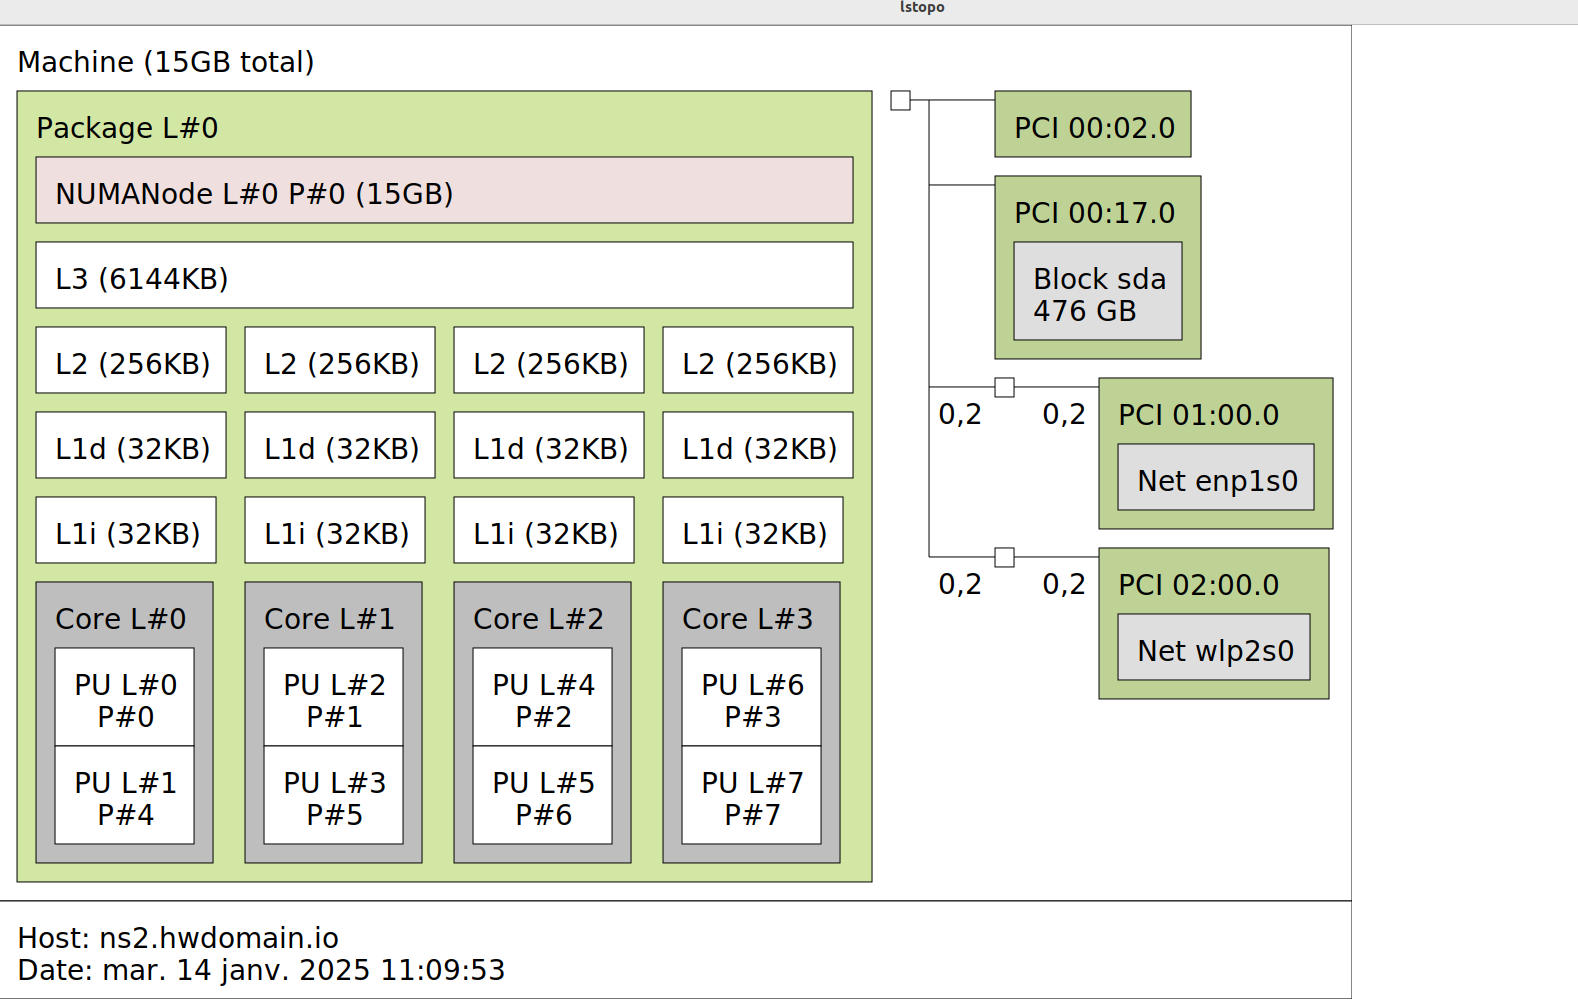
\includegraphics[scale=0.3]{../images/lstopo.png}
      \caption{Résultat de la commande lstopo : Nous pouvons visualiser les tailles des caches}
      \label{tab:ls_topo}
  \end{center}
\end{figure}
\begin{figure}[!h]
  \begin{center}
  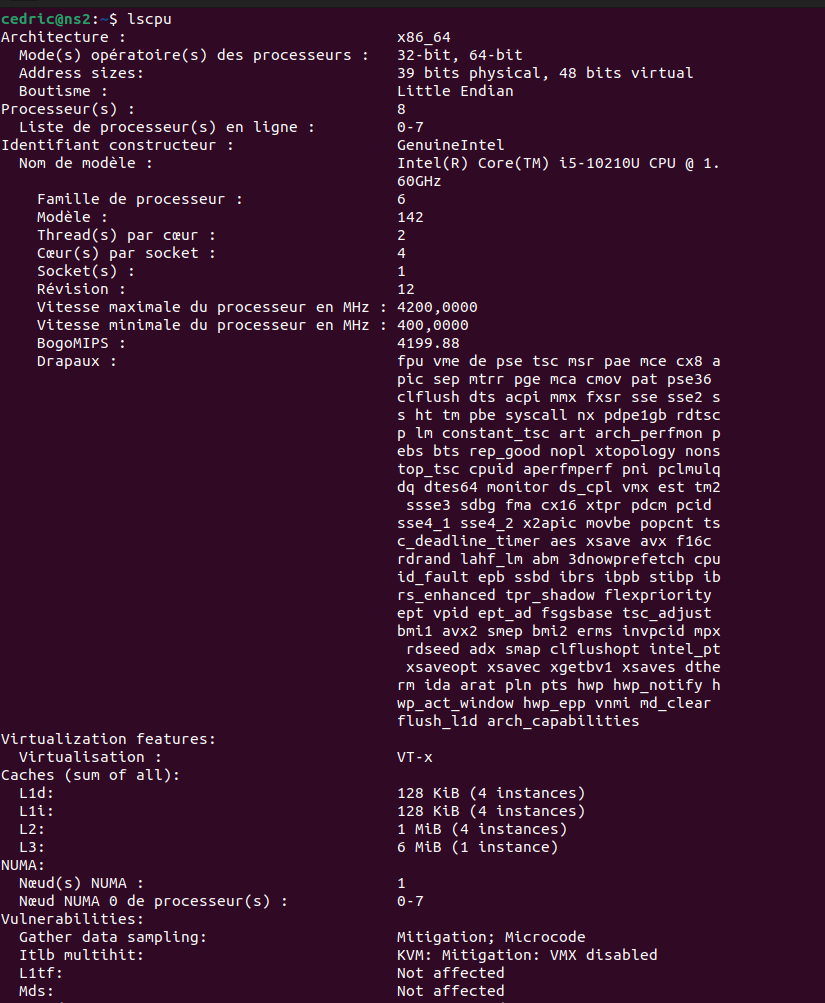
\includegraphics[scale=0.5]{../images/lscpu.png}
  \caption{Résultat de la commande lscpu}
  \label{fig:lscpu}
\end{center}
\end{figure}


\clearpage
\subsection{Informations clés de l'ordinateur}

\subsection*{Contexte d'exécution}
\begin{itemize}[leftmargin=*]
    \item \textbf{Système d'exploitation} : Ubuntu installé en dual boot (natif).
    \item \textbf{Runtime} : Exécution native sur le matériel, sans virtualisation intermédiaire.
    \item \textbf{Avantages du natif} : Meilleure performance grâce à l'absence de surcharge liée à une couche de virtualisation.
\end{itemize}

\subsection*{Architecture et processeur}
\begin{itemize}[leftmargin=*]
    \item \textbf{Architecture} : x86\_64 (64 bits).
    \item \textbf{Modèle du processeur} : Intel(R) Core(TM) i5-10210U.
    \item \textbf{Fréquence} :
        \begin{itemize}
            \item Base : 1.60 GHz.
            \item Turbo Boost : 4.20 GHz.
        \end{itemize}
    \item \textbf{Cœurs et threads} : 4 cœurs physiques, 8 threads (Hyper-Threading).
    \item \textbf{Importance} : Permet une parallélisation efficace avec jusqu'à 8 threads.
\end{itemize}

\subsection*{Cache}
\begin{itemize}[leftmargin=*]
    \item \textbf{L1d} : 128 KiB (4 instances).
    \item \textbf{L1i} : 128 KiB (4 instances).
    \item \textbf{L2} : 1 MiB (4 instances).
    \item \textbf{L3} : 6 MiB (1 instance).
    \item \textbf{Importance} : Réduit la latence d'accès à la mémoire, crucial pour les simulations intensives en calcul.
\end{itemize}
\clearpage
\section{Question 1}

Nous avons attribué un processus à une portion des frames. Chaque processus traite un nombre égale de frames et sauvegarde les images correspondantes
\begin{table}[h!]
    \centering
    \caption{Temps et speedup pour \texttt{movie\_filter}}
    \label{tab:movie_filter}
    \begin{tabular}{@{}cccc@{}}
    \toprule
    \textbf{Nombre de processus} & \textbf{Temps (s)} & \textbf{Speedup} & \textbf{Commentaires}\\
    \midrule
    1 & 26.936 & 1.00 & (version séquentielle)\\
    2 & 35.674 & 0.76 & \\
    3 & 26.968 & 1.00 & \\
    4 & 23.744 & 1.13 & \\
    \bottomrule
    \end{tabular}
    \end{table}
    
    \begin{figure}[h!]
    \centering
    \begin{tikzpicture}
    \begin{axis}[
        width=0.8\textwidth,
        height=0.5\textwidth,
        xlabel={Nombre de processus},
        ylabel={Speedup},
        xmin=1, xmax=4,
        ymin=0, ymax=1.5,
        xtick={1,2,3,4},
        ytick={0,0.5,1.0,1.5},
        legend pos=north west,
        grid=major,
        title={\texttt{movie\_filter}: Speedup}
    ]
    \addplot[
        color=purple,
        mark=triangle
    ]
    coordinates {
        (1,1.00)
        (2,0.76)
        (3,1.00)
        (4,1.13)
    };
    \end{axis}
    \end{tikzpicture}
    \caption{Speedup de \texttt{movie\_filter} en fonction du nombre de processus}
    \label{fig:movie_filter_speedup}
    \end{figure}
\section{Question 2}
\subsection{ Stratégie de parallélisation}

Le but est de doubler la taille des images d’une vidéo (un ensemble de N images) en leur appliquant différents filtres (filtre de flou gaussien, puis filtre de netteté).

\subsection{Stratégie adoptée}

    Découper la liste d’images (les 37 images perroquet, par exemple) en blocs.
    Attribuer chaque bloc d’images à un processus.
    Chaque processus charge, traite et sauvegarde sa portion d’images.

Ce schéma (appelé parallélisation par distribution de tâches) est particulièrement bien adapté pour un ensemble d’images indépendant les unes des autres :

    Peu de communication : chaque processus traite ses images localement, il n’y a pas besoin d’échanger des données entre processus.
    Charge relativement équilibrée : si le nombre d’images est suffisamment grand et que la répartition est équitable, chaque processus réalise une quantité de travail similaire.

\subsection{Pourquoi c’est optimal pour ce problème ?}

    Les images sont indépendantes : on n’a pas besoin de transmettre les bords de l’image 1 à l’image 2, etc.
    Les filtres appliqués (flou gaussien, netteté) se font localement à l’échelle d’une seule image.
    On minimise les communications : la seule étape éventuellement commune est la création d’un répertoire de sortie et/ou la vérification des sommes MD5 (pour la validation).

\section{Observations}

    Pour 2 processus, le temps total (bottleneck) se situe autour de 35 s, ce qui est un peu plus long que la version séquentielle (26-27 s), donc le speedup est < 1.
        Il peut y avoir plusieurs raisons : overhead de MPI, surcoût d’E/S disque, déséquilibre de charge, etc.
    Pour 3 processus, on retrouve un temps d’environ 26-27 s, donc un speedup proche de 1.
    Pour 4 processus, le temps descend à 23-24 s, soit un speedup autour de 1.13.

On constate donc que, dans ce cas précis, le gain n’est pas spectaculaire, voire peut parfois être inférieur à 1 si la charge E/S ou la synchronisation est trop importante. Cela dépend aussi de la taille des images, de la rapidité du disque, etc.
\begin{table}[h!]
    \centering
    \caption{Temps et speedup pour \texttt{double\_size}}
    \label{tab:double_size}
    \begin{tabular}{@{}cccc@{}}
    \toprule
    \textbf{Nombre de processus} & \textbf{Temps (s)} & \textbf{Speedup} & \textbf{Commentaires}\\
    \midrule
    1 & 26.600 & 1.00 & (version séquentielle)\\
    2 & 17.420 & 1.53 & \\
    3 & 17.176 & 1.55 & \\
    4 & 9.960  & 2.67 & \\
    \bottomrule
    \end{tabular}
    \end{table}
    \begin{figure}[h!]
        \centering
        \begin{tikzpicture}
        \begin{axis}[
            width=0.8\textwidth,
            height=0.5\textwidth,
            xlabel={Nombre de processus},
            ylabel={Speedup},
            xmin=1, xmax=4,
            ymin=0, ymax=3,
            xtick={1,2,3,4},
            ytick={0,1,2,3},
            legend pos=north west,
            grid=major,
            title={\texttt{double\_size}: Speedup}
        ]
        \addplot[
            color=blue,
            mark=o
        ]
        coordinates {
            (1,1.00)
            (2,1.53)
            (3,1.55)
            (4,2.67)
        };
        \end{axis}
        \end{tikzpicture}
        \caption{Speedup de \texttt{double\_size} en fonction du nombre de processus}
        \label{fig:double_size_speedup}
        \end{figure}

\section{Question 3}
\subsection{Stratégie de parallélisation}

Ici, on cherche à doubler la taille d’une unique photo (en haute résolution) en appliquant des filtres. Le souci est d’éviter de surconsommer de la mémoire :

    On ne veut pas que chaque processus charge l’intégralité de l’image, car celle-ci peut être volumineuse (plusieurs dizaines ou centaines de Mo).
    On découpe donc l’image en bandes (par lignes, par exemple) : chaque processus ne reçoit qu’une partie de l’image.

\subsection{Pourquoi c’est adapté ?}

    On traite la même image, mais on peut appliquer les filtres localement sur la zone qui nous intéresse, en faisant attention aux bords (si besoin d’un recouvrement).
    Le volume de données manipulées par chaque processus est réduit, on reste dans la limite de la mémoire cache.

\subsection{Optimalité par rapport à la question 2 ?}

    Dans la question 2, chaque processus traitait des images différentes. Ici, tous les processus travaillent sur différentes zones d’une seule et même image.
    L’approche en bandes (ou en tuiles) est nécessaire ici pour ne pas charger la totalité de l’image dans chaque processus.
    On peut dire qu’elle est adaptée (et souvent optimale) pour un traitement d’une seule image, tandis que la question 2 était une distribution par “liste d’images”.

\subsection{ Parallélisation du programme double_size.py}

    On lit l’image sur le processus 0, on la convertit en un tableau.
    On découpe ce tableau en N blocs (un par processus).
    Chaque processus applique les filtres (flou, netteté) sur sa partie.
    On regroupe le résultat final (gather).

\subsection{Courbe d’accélération}


    Version séquentielle : $\approx$26.600 s
    2 processus : $\approx$17.4 s (max) => speedup ≈1.53≈1.53
    3 processus : $\approx$17.2 s => speedup ≈1.55≈1.55
    4 processus : $\approx$9.96 s => speedup ≈2.67≈2.67

On observe un speedup significatif, surtout à 4 processus.
\begin{table}[h!]
    \centering
    \caption{Temps et speedup pour \texttt{double\_size2}}
    \label{tab:double_size2}
    \begin{tabular}{@{}cccc@{}}
    \toprule
    \textbf{Nombre de processus} & \textbf{Temps (s)} & \textbf{Speedup} & \textbf{Commentaires}\\
    \midrule
    1 & 26.584 & 1.00 & (version séquentielle)\\
    2 & 23.372 & 1.14 & \\
    3 & 20.203 & 1.31 & \\
    \bottomrule
    \end{tabular}
    \end{table}
    
    \begin{figure}[h!]
    \centering
    \begin{tikzpicture}
    \begin{axis}[
        width=0.8\textwidth,
        height=0.5\textwidth,
        xlabel={Nombre de processus},
        ylabel={Speedup},
        xmin=1, xmax=3,
        ymin=1, ymax=1.4,
        xtick={1,2,3},
        ytick={1,1.1,1.2,1.3,1.4},
        legend pos=north west,
        grid=major,
        title={\texttt{double\_size2}: Speedup}
    ]
    \addplot[
        color=red,
        mark=square
    ]
    coordinates {
        (1,1.00)
        (2,1.14)
        (3,1.31)
    };
    \end{axis}
    \end{tikzpicture}
    \caption{Speedup de \texttt{double\_size2} en fonction du nombre de processus}
    \label{fig:double_size2_speedup}
    \end{figure}
    \subsection{Stratégie de parallélisation}

    Le principe est similaire (on veut doubler la taille de l’image, mais avec un filtre différent sur la composante V). On découpe toujours l’image en bandes ou en tuiles pour réduire la mémoire nécessaire par processus.
    
        Ici, on applique le filtre F G (flou gaussien) sur H et S, et le filtre F D (différent) sur la composante V.
        Les canaux H, S, V peuvent être traités en parallèle, ou successivement, selon le code.
    
    \subsection{Différences par rapport à la question précédente}
    
        Différence de filtres : on n’applique plus le même masque sur la luminance, on utilise un masque F D (ou un masque 5×5 modifié).
        Surcoût éventuel : le masque 5X5 peut nécessiter plus de calcul qu’un 3×3, et parfois plus de lignes “fantômes” (bordures) pour la convolution.
        Avantage : le traitement H et S est plus léger (flou simple), le traitement V est plus précis.
        Inconvénient : si la communication des bords est nécessaire, on peut avoir un surcoût de synchronisation.

    
        Version séquentielle : $\approx$26.584 s
        2 processus : $\approx$23.372 s => speedup ≈1.14≈1.14
        3 processus : $\approx$20.203 s => speedup ≈1.31≈1.31
    
    Le speedup est moins important que pour double_size.py, ce qui peut s’expliquer par :
    
        Un overhead plus grand,
        Le masque plus grand sur la composante V (ou un autre type de filtre) qui ajoute du temps de calcul,
        Un possible coût plus important dans la distribution/assemblage.
\end{document}